\documentclass{article}
\usepackage{amsmath,amsthm,amssymb,amsfonts}
\usepackage{setspace,enumitem}
\usepackage{graphicx}
\usepackage{hyperref}
\usepackage{natbib}
\usepackage{afterpage}
\usepackage{xcolor}
\usepackage{etoolbox}
\usepackage{booktabs}
\usepackage{pdfpages}
\usepackage{multicol}
\usepackage{geometry}
\usepackage{accents}
\usepackage{bbm}
\usepackage{placeins}
\usepackage{verbatim}
\usepackage{csvsimple}
\hypersetup{
	colorlinks,
	linkcolor={blue!90!black},
	citecolor={red!90!black},
	urlcolor={blue!90!black}
}

\newtheorem{theorem}{Theorem}
\newtheorem{assumption}{Assumption}
\newtheorem{definition}{Definition}
\newtheorem{lemma}{Lemma}
\setlength{\parindent}{0cm}
\geometry{margin = 1in}

\newcommand{\R}{\mathbb{R}}
\newcommand{\ubar}[1]{\underaccent{\bar}{#1}}
\newcommand{\Int}{\text{Int}}
\newcommand{\xbf}{\mathbf{x}}
\newcommand{\Abf}{\mathbf{A}}
\newcommand{\Bbf}{\mathbf{B}}
\newcommand{\Gbf}{\mathbf{G}}
\newcommand{\bbf}{\mathbf{b}}
\newcommand{\one}{\mathbbm{1}}

\newtoggle{extended}
\settoggle{extended}{false}

\title{ECON 717B: PS 1}
\author{Alex von Hafften}

\begin{document}

\maketitle

\begin{enumerate}

\item Roy Model

\begin{enumerate}

\item Why can we normalization $\pi_1 =\pi_2 = 1$?

\bigskip

We can normalize $\pi_1 = \pi_2 = 1$ without any loss of generality because we can change $\mu_k$ to account for non-unit wages:

\begin{align*}
W_k 
&= \pi_k S_k\\
&= \pi_k \exp(\mu_k + \varepsilon_k) \\
&= \exp(\log(\pi_k)) \exp(\mu_k + \varepsilon_k) \\
&= \exp(\log(\pi_k)+\mu_k + \varepsilon_k) \\
&= \exp(\tilde\mu_k + \varepsilon_k) \\
\text{where } \tilde\mu_k &\equiv  \log(\pi_k)+\mu_k
\end{align*}

We don't observe skills, so we can just define the skills distribution with a level shift that accounts for wages.

\bigskip

\item Program to compute the model

\bigskip

See \texttt{run.jl}.  The \texttt{parameters} structure holds parameters and the data structure holds data. The \texttt{simulate\_data} function creates simulated data based on the \texttt{parameters} structure you pass it.

\bigskip

\item Choose parameters such that 60 percent of simulations choose occupation 1

\bigskip

I found $\theta_0 = (\mu_1 = 1.15, \mu_2 = 1.0, \sigma_1 = 0.4, \sigma_2 = 0.5, \rho = 0.25)$ result in about 60 percent of observations choosing occupation 1.  From the formula for the fraction choosing occupation 1 (derived for part g), these parameters analytically result in 60.62 percent choosing occupation 1.  I simulate 1,000 observations and 59.55 percent choose occupation 1.

\pagebreak

\item Write estimator for $\theta$

\bigskip

I use maximum likelihood to derive the estimator. The maximum likelihood estimator is $\hat\theta_{MLE}$:

$$
\hat \theta_{MLE} = \arg \max_{\theta \in \Theta} \sum_{i=1}^N \ln L_i(\theta|X_i, Z_i)
$$

where $L_i$ is the observation-level likelihood function. If the model is correctly specified (which we know holds because this is a Monte Carlo) and some regularity conditions, the $\hat\theta_{MLE}$ is consistent for $\theta_0$:

$$
\hat\theta_{MLE} \to^p \theta_0
$$


I evaluate the likelihood function per observation two different ways.  The first approach uses Julia's built-in approximation for the normal CDF and the second uses simulations. I am interested in both approaches because while the first is ``better" (i.e., it does not introduce simulation error), it can only be done in limited circumstances (e.g., when we can evaluate the likelihood as a function of normal pdfs and cdfs).

\bigskip

I use a Nelder-Mead simplex optimizer to find $\hat\theta_{MLE}$. It works well for the likelihood functions using the built-in normal cdf approximation, but is much slower and performs worse for the simulation-likelihood function.  This makes sense because the former is smooth and the latter has simulation error.

\subsubsection*{Likelihood Function using Built-In Normal CDF Approximation}

For clarity, I use uppercase letters for random variables and lowercase letters for realization of random variables.  For each observation $i$, we observe their occupation choice $d$ and their wage $w$. Thus, the likelihood function for each $i$ is:

\begin{align*}
L_i(\theta| w, d) 
&= 
Pr(W_1 > W_2 , W_1 = w | \theta)^{d} 
Pr(W_2 > W_1 , W_2 = w | \theta)^{1-d}\\
&= 
Pr(W_1 > W_2 | W_1 = w, \theta)^{d} 
Pr(W_1 = w|\theta)^{d} \\ 
&\times
Pr(W_2 > W_1 | W_2 = w, \theta)^{1-d} 
Pr(W_2 = w|\theta)^{1-d}
\end{align*}

Considering each term separately:

\begin{align*}
Pr(W_1 = w|\theta)
&= 
Pr(\pi_1\exp(\mu_1 + \varepsilon_1) = w |\theta)\\
&= 
Pr\Big(\varepsilon_1 = \log\Big(\frac{w}{\pi_1}\Big) - \mu_1 \Big|\theta\Big)\\
&= 
\phi\Bigg(\frac{\log(\frac{w}{\pi_1}) - \mu_1}{\sigma_1}\Bigg)\\
\implies
Pr(W_2 = w|\theta)
&= 
\phi\Bigg(\frac{\log(\frac{w}{\pi_2}) - \mu_2}{\sigma_2}\Bigg)\\
Pr(W_1 > W_2 | W_1 = w, \theta)
&= 
Pr\Big(\pi_1\exp(\mu_1 + \varepsilon_1) > \pi_2\exp(\mu_2 + \varepsilon_2) \Big| \varepsilon_1 = \log\Big(\frac{w}{\pi_1}\Big) - \mu_1, \theta\Big)\\
&= 
Pr\Big(\log \pi_1 + \mu_1 + \varepsilon_1 > \log\pi_2 + \mu_2 + \varepsilon_2 \Big| \varepsilon_1 = \log\Big(\frac{w}{\pi_1}\Big) - \mu_1, \theta\Big)\\
&= 
Pr\Big(\log \pi_1 - \log \pi_2 + \mu_1 -\mu_2 + \varepsilon_1 > \varepsilon_2 \Big| \varepsilon_1 = \log\Big(\frac{w}{\pi_1}\Big) - \mu_1, \theta\Big)
\end{align*}

where $\phi$ is the standard normal pdf.  In this case, we can use the fact that for bivariate normal distributions the conditional distribution is normal:

$$
\varepsilon_2 \Bigg| \varepsilon_1 = a \sim N\Bigg( \frac{\sigma_2}{\sigma_1}\rho a, (1-\rho^2)\sigma_2^2 \Bigg)
$$

So,

\begin{align*}
Pr(W_1 > W_2 | W_1 = w, \theta) 
&= \Phi\Bigg( \frac{\log \pi_1 - \log \pi_2 + \mu_1 -\mu_2 + [\log\Big(\frac{w}{\pi_1}\Big) - \mu_1] - \frac{\sigma_2}{\sigma_1}\rho[\log\Big(\frac{w}{\pi_1}\Big) - \mu_1]}{\sqrt{1- \rho^2} \sigma_2} \Bigg)\\
&= \Phi\Bigg( \frac{\log \pi_1 - \log \pi_2 + \mu_1 -\mu_2 + (1 - \frac{\sigma_2}{\sigma_1}\rho)[\log\Big(\frac{w}{\pi_1}\Big) - \mu_1]}{\sqrt{1- \rho^2} \sigma_2} \Bigg)\\
\implies
Pr(W_2 > W_1 | W_2 = w, \theta) 
&= \Phi\Bigg( \frac{\log \pi_2 - \log \pi_1 + \mu_2 -\mu_1 + (1 - \frac{\sigma_1}{\sigma_2}\rho)[\log\Big(\frac{w}{\pi_2}\Big) - \mu_2]}{\sqrt{1- \rho^2} \sigma_1} \Bigg)
\end{align*}

where $\Phi$ is the standard normal cdf.  So, the likelihood function boils down to:

\begin{align*}
L_i(\theta| w, d) 
&= 
\Bigg[\phi\Bigg(\frac{\log(\frac{w}{\pi_1}) - \mu_1}{\sigma_1}\Bigg)\Bigg]^{d}\Bigg[\Phi\Bigg( \frac{\log \pi_1 - \log \pi_2 + \mu_1 -\mu_2 + (1 - \frac{\sigma_2}{\sigma_1}\rho)[\log\Big(\frac{w}{\pi_1}\Big) - \mu_1]}{\sqrt{1- \rho^2} \sigma_2} \Bigg)\Bigg]^{d}\\
&\times
\Bigg[\phi\Bigg(\frac{\log(\frac{w}{\pi_2}) - \mu_2}{\sigma_2}\Bigg)\Bigg]^{1-d}
\Bigg[\Phi\Bigg( \frac{\log \pi_2 - \log \pi_1 + \mu_2 -\mu_1 + (1 - \frac{\sigma_1}{\sigma_2}\rho)[\log\Big(\frac{w}{\pi_2}\Big) - \mu_2]}{\sqrt{1- \rho^2} \sigma_1} \Bigg)\Bigg]^{1-d}
\end{align*}

\subsubsection*{Simulation-Based Likelihood Function}

Given $\theta$, I simulate $N$ observations.  I split the simulations based occupation choice and I estimate a kernel density for the wages in each occupation.  Then, the likelihood of each observation is:

$$
L_i(\theta|w, d) = \Bigg[\frac{N_1}{N} kde_1(w)\Bigg]^{d} \Bigg[\frac{N_2}{N} kde_2(w)\Bigg]^{1-d}
$$

where $N_k$ is the number of the simulations that choose occupation $k$ and $kde_k(w)$ is the estimate of the kernel density at $w$ for occupation $k$. Importantly, I fix the random seed as I change parameters, so the $\varepsilon_k/\sigma_k$ are the same across calls by the optimizer.

\bigskip

\item Write code to estimate $\theta$ using estimator

\bigskip

See \texttt{model.jl}.  The function \texttt{likelihood} evaluates the observation-level likelihood based using the built-in normal CDF approximation. The function \texttt{log\_likelihood} evaluates the full log-likelihood.  It has an option to run it using each method for evaluating likelihood.  The function \texttt{mle} runs the optimization step.  I use a scaled and shifted logistic function to make sure $\rho$ is confined between -1 and 1.

\pagebreak

\item Plot identification figures

\bigskip

I plot identification figures for each method of computing likelihood.  I plot a contour figure where $\mu_1$ changes on the x-axis and $\rho$ changes on the y-axis and the color indicates the log-likelihood. The orange dot is the true value of the parameters and the green dot is the ML estimates. In addition, I plot the log-likelihood as we change one parameter and holding the other fixed at both its ``true" value (blue line) or the MLE estimated value (orange line).  The true value of the parameter is shown by the purple line and the ML estimate is the green line. We can see that $\mu_1$ is more sharply identified than $\rho$.  The log-likelihood function is more curved as you change $\mu_1$.  The $\hat\mu_1$ is very close to the true value, but $\hat\rho$ is further away from its true value.  As expected, the simulation-based likelihood function added noise.  The effect for $\mu_1$ is not so bad, but there is much more noise and a much less accurate estimate for $\rho$.

\subsubsection*{Likelihood Function using Built-In Normal CDF Approximation}

\begin{center}
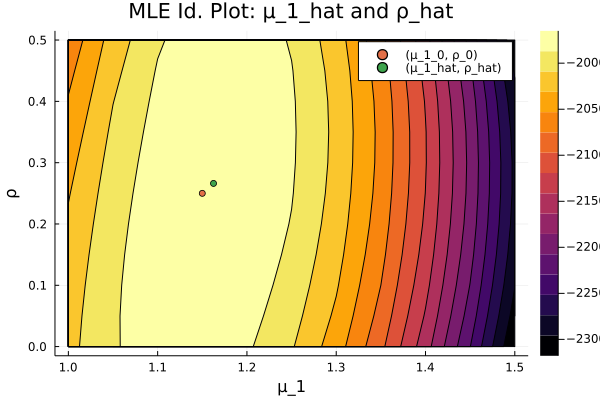
\includegraphics[scale =0.5]{q_f_3d}
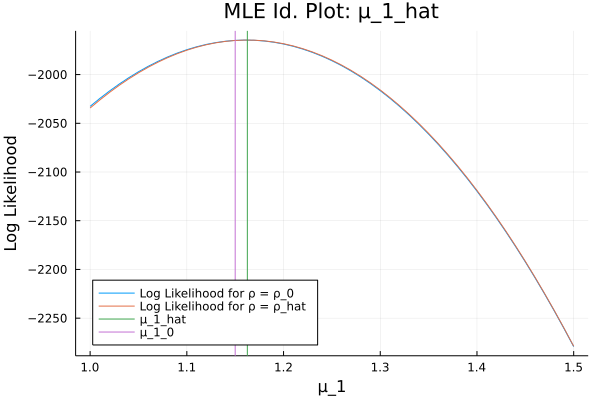
\includegraphics[scale =0.5]{q_f_mu_1}
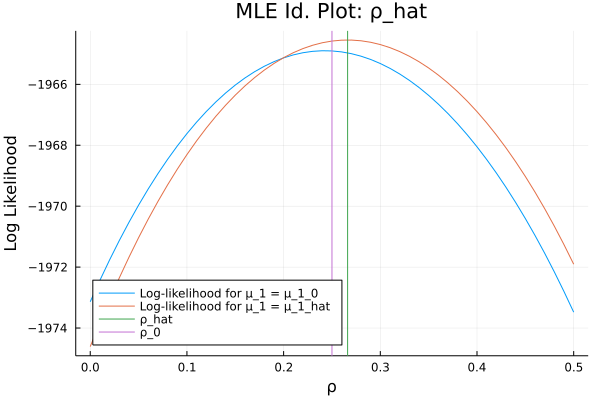
\includegraphics[scale =0.5]{q_f_rho}
\end{center}

\subsubsection*{Simulation-Based Likelihood Function}

\begin{center}
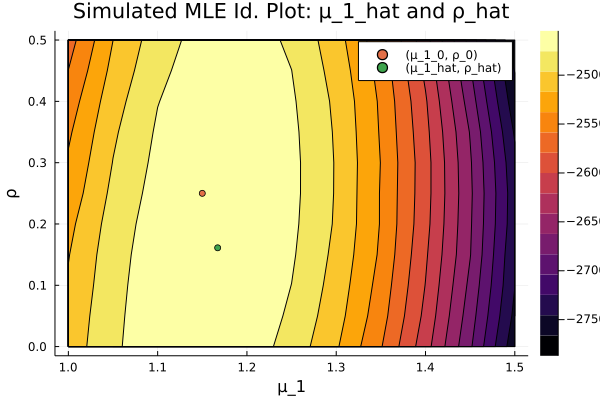
\includegraphics[scale =0.5]{q_f_3d_s}
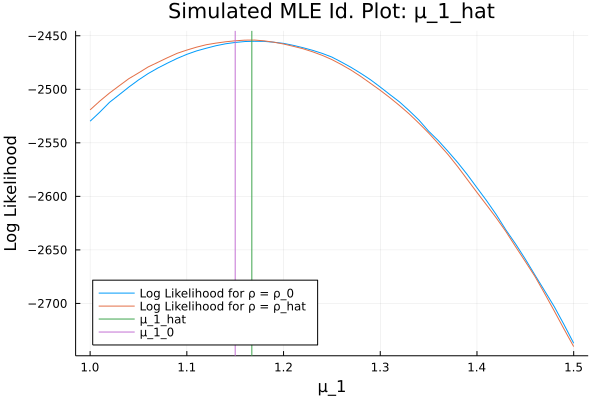
\includegraphics[scale =0.5]{q_f_mu_1_s}
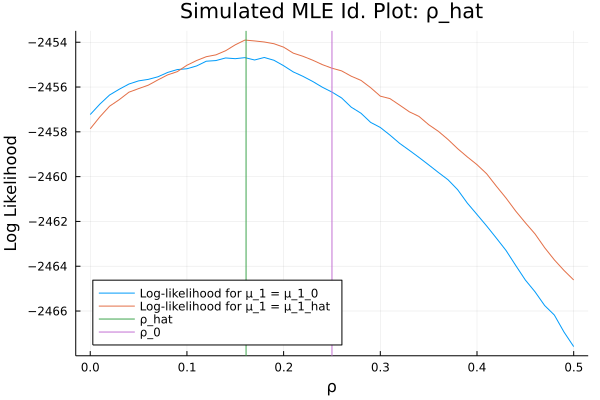
\includegraphics[scale =0.5]{q_f_rho_s}
\end{center}

\bigskip

\item Table of parameters and model fit

\bigskip

The fraction of agents that choose occupation 1 implied by the model is:

\begin{align*}
Pr(W_1 > W_2)
&= Pr(\pi_1 \exp(\mu_1 + \varepsilon_1) > \pi_2 \exp(\mu_2 + \varepsilon_2)) \\
&= Pr(\log(\pi_1) +\mu_1 + \varepsilon_1 > \log(\pi_2) + \mu_2 + \varepsilon_2) \\
&= Pr( \varepsilon_2 - \varepsilon_1 < \log(\pi_1) + \mu_1 - \log(\pi_2) - \mu_2) \\
\text{where } 
\varepsilon_2 - \varepsilon_1 &\sim N(0, \sigma_1^2 + \sigma_2^2 - 2 \rho \sigma_1 \sigma_2)\\
\implies
Pr(W_1 > W_2) &= \Phi\Bigg(\frac{\log(\pi_1) + \mu_1 - \log(\pi_2) - \mu_2}{\sqrt{\sigma_1^2 + \sigma_2^2 - 2 \rho \sigma_1 \sigma_2}}\Bigg)
\end{align*}

For the other model fit moments, I just simulate a 100,000,000 observations for each parameter vector and compute the data moments because I was running into troubles deriving an explicit formula.\footnote{ My progress on the expected value of observed $W_1$:

\begin{align*}
E[W_1 | W_1 > W_2]
&= 
E[\pi \exp(\mu_1 + \varepsilon_1) | W_1 > W_2] \\
&= 
\pi \exp \Big(\mu_1 + E[\varepsilon_1 | W_1 > W_2] + \frac{1}{2} V[\varepsilon_1 | W_1 > W_2]\Big) \\
E[\varepsilon_1 | W_1 > W_2] 
&= 
E[\varepsilon_1 | \pi_1 \exp( \mu_1 + \varepsilon_1) > \pi_2 \exp( \mu_2 + \varepsilon_2)] \\
&= 
E[\varepsilon_1 | \log \pi_1 + \mu_1 + \varepsilon_1 > \log \pi_2 + \mu_2 + \varepsilon_2] \\ 
&= 
E[\varepsilon_1 |  \varepsilon_1 > \log \pi_2 - \log \pi_1 + \mu_2 - \mu_1 + \varepsilon_2] \\
&= ... 
\end{align*}

} I tried simulating 20 percent more simulations and my estimates did not change, so I think this number of observations were sufficient for at least three significant digits.  

\bigskip

The table asked for in the problem set is below.  The first column is the simulated data moment and the second column are these moments at the parameters estimated with MLE.  Everything is quite close.

\bigskip

\begin{center}
\csvautotabular{q_g_table_1.csv}
\end{center}

\bigskip

I expanded the previous table to include some addition information.  The first column are these moments at the ``true" parameter.  The second column are the data moments. The difference between these columns stems from simulation error.  The third column are the MLE estimates.  The difference between these columns is due to the estimation error.  The fourth column are these moments using the parameters from the simulation-based MLE estimates.  The difference between these columns is due to using simulations in the estimation.

\bigskip

\begin{center}
\csvautotabular{q_g_table_2.csv}
\end{center}

\bigskip

\item Minimum wage counterfactual

\bigskip

I run the counterfactual for a range of minimum wages in occupation 1 from 0.0 to 12.0, at which over 99.9 percent of simulations choose occupation 1.  I plot the fraction choosing occupation 1, the average observed wage in each occupation, and the standard deviation of wages in each occupation.  I then focus on 2.9, which is the minimum wage in occupation 1, so that 70 percent of simulation choose occupation 1.

\begin{center}
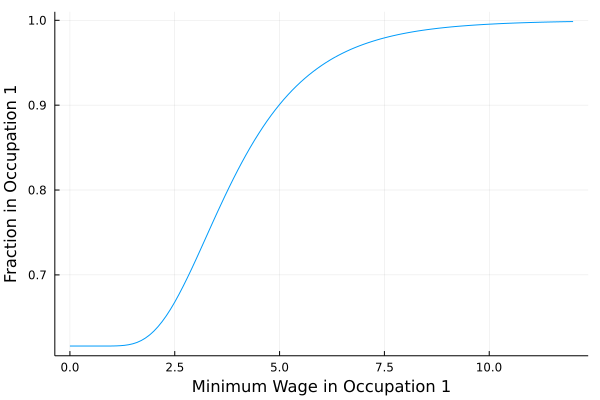
\includegraphics[scale =0.5]{q_h_fraction}
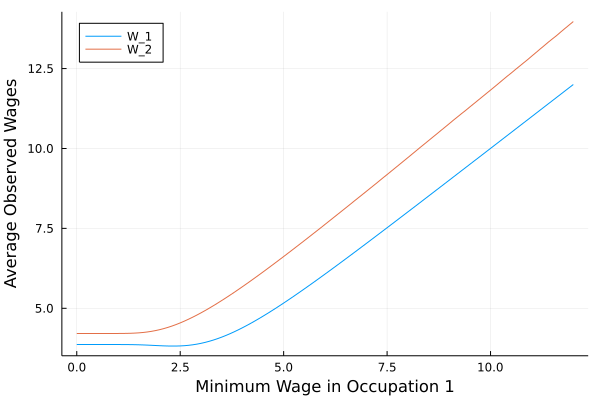
\includegraphics[scale =0.5]{q_h_average}
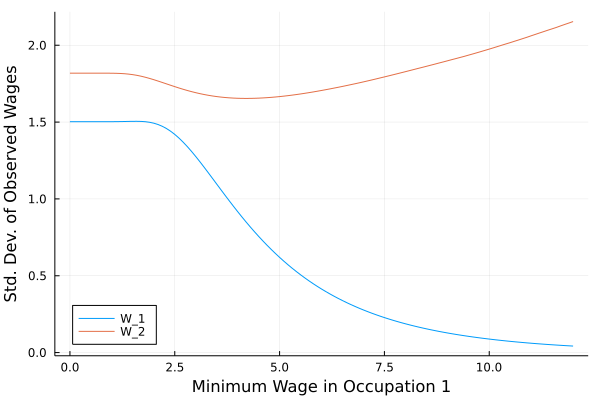
\includegraphics[scale =0.5]{q_h_std_dev}
\end{center}

\begin{center}
\csvautotabular[respect underscore=true]{q_h_table.csv}
\end{center}

\end{enumerate}

\end{enumerate}


\end{document}